% !TEX root = ../main.tex


\chapter{Approach}
After we learned the underlying concepts, we can go on with the actual task.

In this chapter it is shown how the initial rust code is translated and analysed.
We will see that the rust compiler has interfaces that we can use to reduce our effort,
and that it creates an intermediate representation that fits our needs nicely.
We will work out a translation for the elements of this intermediate representation, 
and discuss the format that we will translate into.
Finally we will discuss how we can use a model checker to find deadlocks in some simple test programs.
%TODO: überleitungssatz?

\section{Rust Compiler}
\label{app_rust}
There are basically two options to translate rust into Petri-Nets:
\begin{enumerate}
    \item write an own translator or,
    \item use something existing.
\end{enumerate}
Writing an own translator means total control over the process.
Features can be added iteratively as needed and data structures can be designed efficiently for this special perpose.
However, this would result in a new compiler for rust which eventually has to cover every language feature;
Including some difficult ones like macro expansion and generics.
Features that someone already implemented, spending a fair amount of thought in the process;
Backed by a large community;
Over several years.
Resulting in a compiler that is openly available under an open source license\cite{rustc}, with a maintained documentation\cite{rustc-guide}\cite{rustc-doc}.
And even though learning how this complex compiler works, and where to find the relevant parts for this project is also difficult, it seems to be time worth spend if we are able to skip learning and implementing difficult features.
For this reason this project is based on the rust compiler `rustc'.
So lets see how its basic structure looks like.

The rust compiler does have several phases and a variety of intermediate representations \cite[Chapter 2.1]{rustc-guide}:
\begin{enumerate}
    \item In the first phase rust source files are parsed to an abstract syntax tree (\textbf{AST}) that matches the original syntax closely.
    \item In the second phase implicit information is expanded. This includes for example macros and identifier names.
    \item Phase three lowers the AST to a simpler form called high-level intermediate representation or \textbf{HIR}.
    The HIR still is quite similar to normal rust syntax but some structures are normalised so that code analysis is easier. 
    For example for loops are rewritten to simple endless loops with break conditions.
    \item The fourth phase executes some static analysis on the HIR.
    Things like type checking and encapsulation verification is done on this representation.
    \item Another representation is generated in phase five: the mid-level intermediate representation (\textbf{MIR}).
    Now we leaving the tree structure and switching to a graph.
    MIR is based on a control-flow graph \cite and language features are reduced to a minimum.
    There is only one type of loop and branches respectively (only gotos instead of ifs or pattern matching).
    Additional static analysis is done on the mir level,
    like rusts borrow checking, as well as further optimization.
    \item Phase six lowers the MIR to the rust independant LLVM\cite intermediate representation.
    LLVM IR is a low level representation that is close to assembly language.
    Optimization for this representation can now be done for the code resulting in several object files.
    \item In the last phase the object files are linked into a complete binary executable.
\end{enumerate}
But wich phase is best to intercept to translate the current intermediate representation into petri nets?

\section{Interception strategie}
\label{app_intercept}
After deciding to use the rust compiler as basis for this work, we need to determine the phase we want to intercept the default compilation to translate to our own target.
A suitable location makes use of the most possible compiler features with the least amount of translation effort.

We want to skip basic features like name resolution as we need this feature ourselfs and surely won't improve it by a reimplementation.
Also code generation, including macro and generics expansion, should be handled by the compiler.
They just produce more rust code that we will treat anyway.
But after expansion, no code generation syntax will remain and we can simply ignore this feature.

More optional for our use are the static analysis features like type checking and borrow checking.
Though, we want to use their assumption, we do not depend on them actually being checked, since nobody will ever run a rust program that did not go through the complete compilation process.
So it is quite safe to assume that nobody will do model checking on a program that won't compile.
However, we still can enforce those invariants if we run the static analisis anyway and abort on errors.
This prevents time consuming runs for programs that cannot be build.

A compiler feature that \textit{can} greatly ease our effort is the lowering of the representation.
After all that means that several high level language features are reduced to less low level features.
Which in turn means less features we have to cover with our implementation.
We don't want to go to low though, since lower representations might prevent us from exploiting assumptions that are hidden in the translation process.
We also probably want to avoid a machine dependant representation.
To verify generic rust programs and not the peculiarities of a single machine.
This might be debateable though.

Lastly we want to make use of all optimizations we can.
Especially optimizations that reduce the code (and resulting net) size.
So features like constant propagation and dead code elimination would be nice to have to reduce the limit of state explosion.
At least a little bit.

Looking back an the rust compiler phases with those thoughts in mind, the seemingly best place we can intercept is between phase five and six.
After borrow checking and optimizations on the MIR.
Here, all code was expended, all rust specific static analisis and optimization was done and all unnecessary language features where reduced to a minimal set of instructions.
And since MIR is a graph representation as well as petri nets, a mapping should be relatively straight forward.
More so if we consider that MIR represents control flow quite closely as petri nets do.
Also we avoid the still lower level and rust independent LLVM IR and the machine dependent object files. 

\section{Mid-level Intermediate Representation (MIR)}
\label{app_mir}
%TODO: examples examples examples

Now where we pinned down MIR as the intermediate representation to use, it is helpful to understand how it is structured.

\begin{figure}
    \centering
    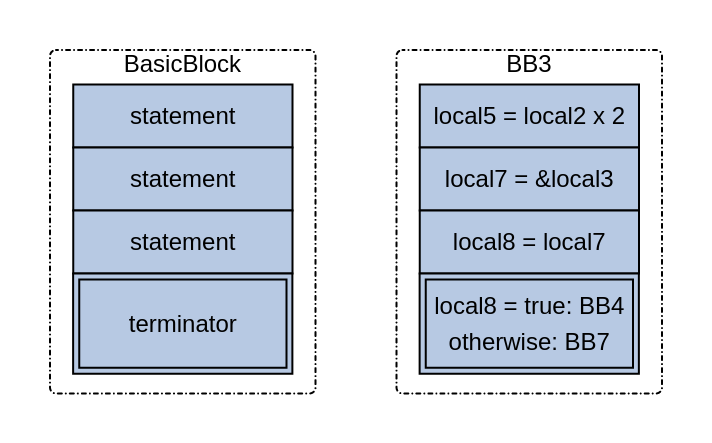
\includegraphics[width=.7\textwidth]{../diagrams/BasicBlock.png}
    \caption{
        Structure of a basic block. 
        Several chained statements with a single trailing terminator.
        The terminator can redirect control flow to other basic blocks.
        In this example BB3 branches to BB4 or BB7 depending on the value of local8
        }
    \label{mir_bb}
\end{figure}

\begin{figure}
    \centering
    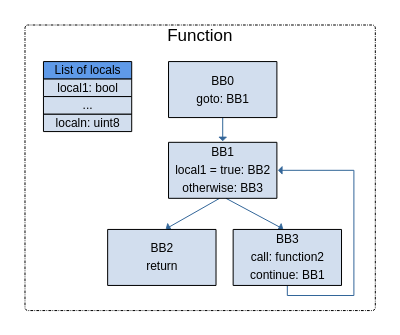
\includegraphics[width=.7\textwidth]{../diagrams/Function.png}
    \caption{
        Example of a functions internal control flow.
        The statements of the basic blocks are omitted as they don't affect control flow.
        A function has a list of locals that are accessible on the stack.
        Each local has an associated type.
        Functions always start with the first basic block (BB0 in this case).
        This function either returns to the calling function in BB2
        or calls `function2' in BB3.
        When function2 returns, control flow continues in BB1.}
    \label{mir_fn}
\end{figure}

As mentioned before, MIR is derived from control flow graphs\cite[chapter 2.17]{rustc-guide}.
It consists of several \textbf{basic blocks} which are interconnected with directed edges.
Each basic block consist of any amount of non branching \textbf{statements} and a single -- possibly branching -- \textbf{terminator}.
All statements in a single basic block are executed sequentially.
Between those, no branching can occur in or out.
Only terminators can redirect the control flow.
They are the ones that represents conditional execution (i.e. if-then-else constructs) or jumps to other basic blocks (including loops).

Data in MIR is represented as \textbf{locals} and \textbf{places} (not to be confused with petri-net places).
Places represent any kind of memory location, whereas locations are conceptually located on the stack.
This means that a location can also be represented as a place, but places are not necessarily locations.
Statements work on these data representations.
The most prominent type of statement is an assignment that assigns an \textbf{rvalue} derived from an expression to a memory location -- meaning a place.
Also based on the data terminators can direct control flow.
Which branch the program takes might depend on the value a place currently holds.

It is also important to know that each function has a separate MIR representation.
Calling other functions is an action done by a call-terminator.
They can direct control flow to a subroutine that is executed until a return-terminator is hit.
After that the calling function resumes execution at a previously defined basic block.
An important note is that the functions in a call are referenced by name and not with an edge in the graph (this results in the separate MIR representation for each function).
This approach ensures that recursive function calls are kept simple.

Besides the specific kinds of statements and terminators, this is the general concept for the MIR graph.
A more detailed view would be of little help since it would get very close to the actual implementation.
Implementation details, however, are frequently changing;
In fact during this work it changed multiple times breaking the code.
A circumstance that is communicated by the compiler team and needed because a too stable API would restrain the compiler development process.


\section{Translation}
\label{app_trans}
After we saw how the MIR graph is structured, we can try to find a translation to Petri-Nets. This will include some more details and edge case we have to consider.

\subsection{Entry Point}
\begin{figure}
    \centering
    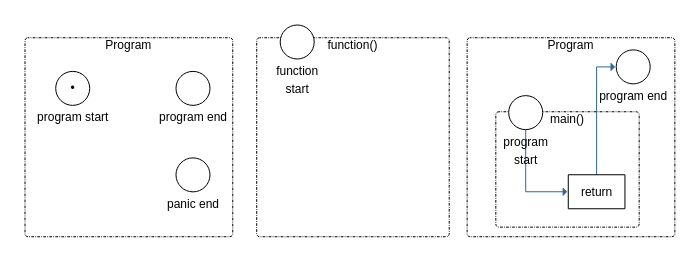
\includegraphics[width=.9\textwidth]{../diagrams/basic_program.png}
    \caption{
        Stubs for programs and functions, and a minimal terminating program.
        A program has a start and an end place.
        The start place holds a token, as program execution begins there.
        If a program terminates successfully the program end place is marked.
        A termination caused by a panic marks only the panic place.\\
        A function has a distinct starting place (it always starts at the first basic block).
        But there is no end place, as functions can be left by any terminator.\\
        The shortest possible (terminating) program has an empty main function.
        Program start place and main function start place are one and the same place.
        Empty functions have no basic block in MIR, so we have to add an artificial transition to leave the function.
    }
    \label{program_blocks_trans}
\end{figure}
The will start with the most abstract view on our translation: the whole program.
A program is something that typically has a beginning end an ending.
We can model this with a \textbf{program start} and an \textbf{program end} place that every program has.
Depending on the program they are interconnected somehow.
The sole exception are programs with a diverging main function -- where the main function ends in an endless loop.
In this case start und end place will not be connected, but an unconnected end place does not harm either.
In rust a second end place for panics -- the \textbf{panic end} place -- is a helpful addition.
This place will be marked then the program terminated unsuccessfully after a panic was raised.
A circumstance that might be helpful to distinguishing in verification runs.
Finally the program start place needs to be marked with a token.
We will later see that this token also indicates the first statement to execute and that it virtually moves from statement to statement acting like a program counter (even though petri net tokens do not move semantically but rather be consumed and produced).

Although these are all the basic features shared by every program, we still have to look a little closer on the semantics of the program start place.
This place is a bit ambiguous since, in practice, the main function is not wat is executed first.
Usually programs have a `runtime' that is initialized before main() is called.
These setup static memory and initialize language specific features, among other things.
And even though low level languages like rust or c hove a small runtime, they still have one.
Now we have to decide if this runtime should be considered for Petri-Net translation.
After all it is part of the finally executed binary.
On the other hand it is platform dependent code that is independant from the actual program semantics.
And there is another problem in starting in the pre main code.
It turns out that the MIR for that part is not completely available in every compiler version.
It is possible to get the missing parts subsequently but it complicates the translation process unnecessarily.
Additionally, we previously argued for a platform independent approach already in chapter \ref{app_intercept}.
It would be inconsistent to detach from that agenda now.
So, because of these reasons we decided to skip the pre main() code and start translating programs with the actual main method.

\subsection{Functions}
After we modeled the important features of a program, we can look on the next important path that a program consists of.
Control flow wise these are functions.
As in most other imperative languages rust programs have a main function that wrap all its functionality (excluding the runtime as discussed in the previous section).
The main function can call other functions that inturn can call additional functions, and so on.
When executing a program the called functions are organized on a stack called `call stack'.
When a new function is entered a new stack frame is pushed on the stack including information like function arguments and local variables.
On leaving a function it is removed from the stack deallocating memory the frame occupied.

In MIR calling and returning from functions is done in a basic block terminator and can occur arbitrarily often.
Considering this behavior in a function model would be of no help, leaving just the start place as a feasible similarity between functions.
A function that is called always begins its execution there.
And it will always be identical to the start place of the first basic block.

So, from a modeling perspective functions are not the decisive abstraction.
But if we consider the translation process they get more important.
The rustc interface for MIR works per function.
This means that it is not possible (at least no obvious one) to get the MIR from a whole program but only from single functions.
A likely explanation for this design choice is that a lot of context information switches with functions.
For example every functions starts with basic block zero and increases the count for the following.
Local variables are also indexed with some of them having a special meaning.
The first being the functions return value followed by variables for all function arguments.
If we want to translate a program we have to keep this structure in mind.
In our implementation we have done this virtually by an own call stack.
We traverse the program function by function.
Every time we encounter a function call terminator we try to translate the called function and return wre we left if we are done.
On the new call the context is switched to the new variables and basic blocks, and the return semantics is stored.

However, this approach has some implications:
\begin{enumerate}
    \item If the same function is called multiple times in the program, it is also translated multiple times.
    Although, this can probably avoided with an intelligent function cache this approach is sufficient for a proof of concept.
    \item The far more extensive implication are the voided recursion capabilities.
    If we encounter a recursive function with this strategie, we will be trapt in an endless loop.
\end{enumerate}
Actually recursion is a feature that can never be achieved with low-level Petri-Nets, as it data model cannot be mapped correctly.
How often a recursive function is called depends on the data it is called with and cannot be known at compile time.
In normal program execution functions are just pushed on a new stack frame until it is resolved (the base case is called for all recursive calls) or the stack overflows.
Most relevant programs will be still executable.
But we cannot model this stack like behavior in low-level Petri-Nets because we cannot get additional memory.
All memory we have is that we know of at compile time.
And we cannot reuse the places of a function for different recursion levels as we can not distinguish the tokens from the recursion levels.
We could just remodel each recursion level again and again to a fixed recursion level.
However, this would impact the verification results, since a property might change for programs with different maximum recursion depths.

A solution to this problem can be high-level petri nets, where we can distinguish between tokens.
There we could reuse places from the same function by annotating tokens with the corresponding recursion level.
We won't go into detail of this approach, though, since this work is based on the low-level semantics.
We will just have to accept that we cannot translate recursive functions for the time being.

\subsection{Memory}
To translate a rust program we cannot focus only on flow.
We also need a valid representation of data.
Unfortunately, as mentioned before, data is complicated to model in low-level petri nets.
With only the concept of bare tokens, we can only model finite memory space and even if we do, modeling every state of every possible variable would bloat our net terribly.

To stay in the realm of low-level nets we have need to abstract from variable states.
In principle a Petri-Net place already is something that holds data: a set of tokens.
If we interpret a place as a memory location and a token is data, though we loose a lot of information, however, we still can analyse the program flow.
Additionally, this representation resonates well with a possible high-level extension where the token can be annotated with the current value of a variable.
So, to keep it simple we represent a memory location as a single place with a single token.
And we `read' from memory with a transition that consumes the token, while also producing a token.

Now in many programing language there are different concepts of memory that behave differently, and rust is no exception.
Basically we can distinguish between four different concepts:
\begin{enumerate}
    \item \textbf{Constant memory space}: The size of the constant space is known at compile time and the values of this space do not change during runtime (hence the name).
    The values of all constants are compiled into the executable and no computation is needed to get them.
    \item \textbf{Static memory space}: Like in the constant space, the size of the static memory space is known at compile time.
    The big difference is that data the static space can change during runtime.
    So during program startup, a fixed amount of memory is allocated and all static variables are initialized.
    Later they can be used rather similar as normal variables. With some rust specific constrains that we will not discuss here, as they are not important for Petri-Net translation.
    \item The \textbf{Stack}: there the size is known for each stack frame (function call).
    This is the combined size of all local variables a function needs for execution.
    If a function is called a now frame is pushed to the stack and if the function terminates the frame is removed.
    Since the last pushed frame will be the first to be removed (LiFo - Last in, first out), the stack can be managed without data fragmentation.
    \item The \textbf{Heap}: which is the place there every remaining memory goes.
    A dynamic variable, there the size cannot be known at compile time needs to allocate memory on demand at runtime.
    If the memory is not needed anymore, it will be deallocated and the again free space can be reused.
    Since both allocation and deallocation are on demand, this can introduce memory fragmentation, since the size of the holes is not uniform.
\end{enumerate}

The most prominent concept on the MIR layer is the stack.
Every part of the MIR is associated with a function which has a set of local variables (locals).
The current state of a local variable is changed by statements.
This includes the values the variable can be assigned to as well as information about variable liveness.
Each local starts in an uninitialized state until a statement is called to set it `storage live'.
A living variable can be assigned to arbitrary values (the type allows) as long as it is needed.
Afterwards a statement sets the variable `storage dead' to indicate that it will not be used again in this function call.
We can model this behavior with three Petri-Net places for each local: one place for the uninitialized state, one for the living state there the variable can be used and one for the dead state.
The first active state will be `uninitialized' so this one must be marked with a token initially.
The unique `storage live' and `storage dead' statements (which are special statements generated for the MIR) have to be called to traverse the three states.
They will consume a token from the previous state and produce one on the next.
This enforces that data access can only be done if a token is on the live place.
This way we can later verify if the liveness invariants are met.

Heap and static space is hidden behind local variables.
For example we can access a value on the heap by dereferencing a pointer we stored in a local.
In MIR this is done with a projection from a local that describes wich part of the local is used;
Which field of a struct, which index of an array or if we dereference the local for example.
This information is stored implicitly as MIR-place on which statements can operate.
Unfortunately this projects is hard to impossible to model.
Especially pointer dereferencing is a problem since the memory model is handled by the operating system at runtime.
But for all these projections the source -- the initial local -- is known.
If we use a projection in a statement we can interpret this as an access to the initial local.
Again we loose some information here in exchange for a manageable design.

What is much easier to model is the space for constant variables.
They behavior is close to locals that live for the entire runtime.
So they do not need any uninitialized or dead place, just a place that represents the current value.
In fact we can model the whole constant space as a single Petri-Net place, where every access is done with different transitions.
Where is no data manipulation anyway.
And again this approch resonates well with a possible high-level petri net extension where every accessing transition produces token with the corresponding constant values.

In conclusion we need two models for memory access: a a set of place for each local variable with uninitialized, live, and dead place, and a single place that represents the whole constant memory space.
Memory is accessed and modified in statements and if we have to handle heap space we can hide this behind an access of a local variable which is projected to other memory space that we are unable to control (or model).
Before take a deeper look on the memory using statements next we will see how we can model the basic blocks that contains the statements.

\subsection{Basic Blocks}
It is essentially a container for a sequential part of a program; 
With an entry point and an exit point.
On exit, program flow can be redirected to one or more other basic blocks (redirections to other functions will again  start at a basic block).

Consequently, in a Petri-Net model, a basic block has an entry place and an exit place.
These are bound to the containing statements, where the basic blocks entry place corresponds to the first statements entry place and the basic blocks exit place corresponds to the last statements exit place.
The terminator is modeled by one or more transitions that are connected to the end place to another basic blocks start place.

\subsection{Statements}
\begin{figure}
    \centering
    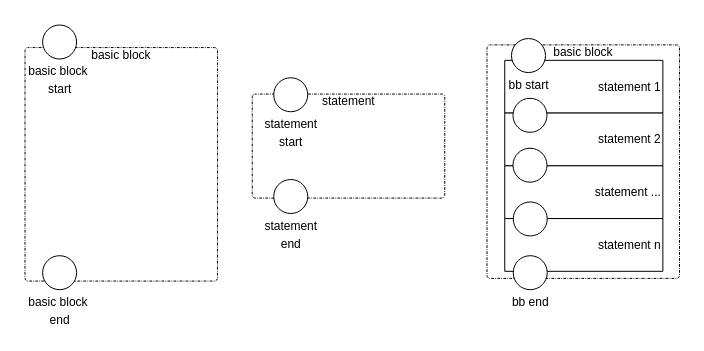
\includegraphics[width=.9\textwidth]{../diagrams/basic_blocks.png}
    \caption{
        The structure of basic blocks and statements.
        Basic blocks as well as statements have a distinct start and end place.
        The start place of the first statement is identical with the basic block start place.
        The same is true for the lasts statements end place and the basic block end.
        Also the end place of a leading statement is the start place of the following statement (illustrating the sequential nature of statements).
        Terminators are represented entirely by transitions that are not pictured here, as they are typically linking to other basic blocks.
    }
    \label{basic_block_trans}
\end{figure}A basic block does not have many features of its own.
Statements are the part of the MIR that change data.
There are several different kinds of statements;
How many and how they are structured depend on the exact kind of the statement.
Additionally, some of them are not used in every compiler phase.
For example a MIR statement named `FakeRead' is used for static analysis but removed in a later optimization phase when the sanity was satisfied.

The general structure of the different statements, however, is always rather similar.
In Petri-Net terms, they have a starting place, a transition that manipulates some data places and an end place.
If two statements succeed each other, the first transitions end place will be the seconds transition start place.
Similarly, the start place of the first statement in a sequence will be shared with the start place of the surrounding basic block
Likewise the end place of the basic block is shared with the end place of the last statement.
The statement transition will consume a token from the start place and produce a token on its end place.
Additionally, the transition will consume and produce data places to resemble a manipulation of this data.
As mentioned earlier the actual data is transparent in the low-level Petri-Net model but might be added in a possible high-level model.

As an example for the data manipulation we can look at the three most important statements: `StorageLive', `StorageDead' and `Assign'.
\begin{itemize}
    \item The \textit{StorageLive} statement consumes a token from the \textit{uninitialized} place of a local variable, and produces one on its \textit{live} place.
    \item The \textit{StorageDead} statement consumes a token from the \textit{live} place of a local variable, and produces one on its \textit{dead} place.
    \item An \textit{Assign} statement in the language semantics, evaluates an expression and assigns the result to a memory location (lvalue).
    In Petri-Net semantics it consumes a token from the lvalues live place and all live places that are involved in the expression.
    Simultaneously new tokens are produced on all of them (one per involved place).
    This means that no assign statement can be executed until the corresponding locals are initialized with a storage live statement or after the local was retired with a storage dead statement.
\end{itemize}

\begin{figure}
    \centering
    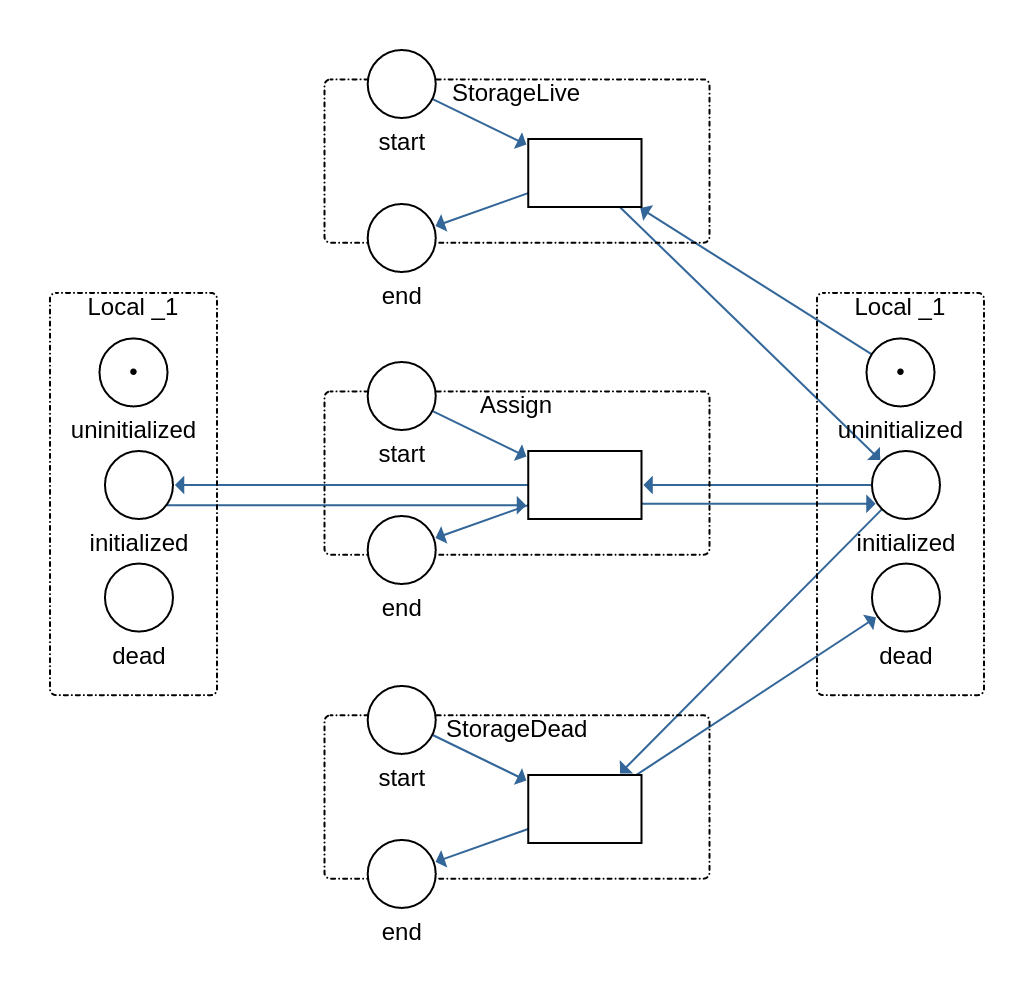
\includegraphics[width=.9\textwidth]{../diagrams/StatementsNet.png}
    \caption{Three kinds of statements (unconnected)}
    \label{statements_net}
\end{figure}

With the virtual movement of a token from one statements start place to another we modeled a marking mechanism for the currently active instruction (meaning a statement or terminator).
If we would simulate the resulting Petri-Net (except at program start and end) we always have a token on exactly one start place of a single instruction.
This instruction will be the next one to be executed and afterwards a new one will be marked.
This property is very close to a \textit{program counter} in CPU's which stores the address of the instruction that will be executed next.
This next instruction might just increment the pointer (in sequential parts) to mark the subsequent instruction as active or manipulates the pointer to jump to a totally different instruction.
This is a convenient similarity since it increases confidence that the Petri-Net actually models something that is similar to an execution semantics of a real program.

Next we see how jumps work in our Petri-Net model.

\subsection{Terminators}
After we covered the strict sequential part of our program we will now discuss the jumping and branching terminators.
They too have a common structure:
Every terminator has at least one transition which consumes a token from a basic block ends place and produce a token on a basic blocks start place.

The MIR representation again has different kinds of terminators. Here is a list with the most important ones:
\begin{itemize}
    \item The most basic \textit{Goto} terminator has a single transition.
    It connects two basic blocks inside of a single function.
    \item The \textit{SwitchInt} terminator implements a conditional branch to multiple other basic blocks.
    A branching path can only be taken if its condition is met.
    However, the last path acts as an \textit{otherwise} branch that will be taken if there is no other valid path.
    As the Petri-Net representation is used for model checking we always consider every possible branch.
    As a result we can ignore the condition and just connect all involved basic blocks with a transition.
    \item The \textit{Call} terminator connects basic blocks of different functions.
    It also encodes function arguments and the basic block to continue after the called function returns.
    We have to remember this information for the translation (especially the arguments),
    And have to make sure that we reuse their locals in the called function.
    Also function calls might panic and if they do execution continues on a separate basic block.
    \item The \textit{Return} terminator is the return path from a successful function call.
    Here the current basic block is connected with the one that is encoded in the Call terminator.
    \item The \textit{Resume} terminator is the return path from an unsuccessful function call.
    This terminator is connected with the panic basic block that is encoded in the function call.
    \item The \textit{Assert} terminator branches depending on a condition.
    If the condition evaluates as expected -- normal execution flow continues, and if it does not -- a panic is started on a separate path.
    Again, in the Petri-Net we always consider both cases so we can safely ignore the condition and just model both paths with a transition.
\end{itemize}

\begin{figure}
    \centering
    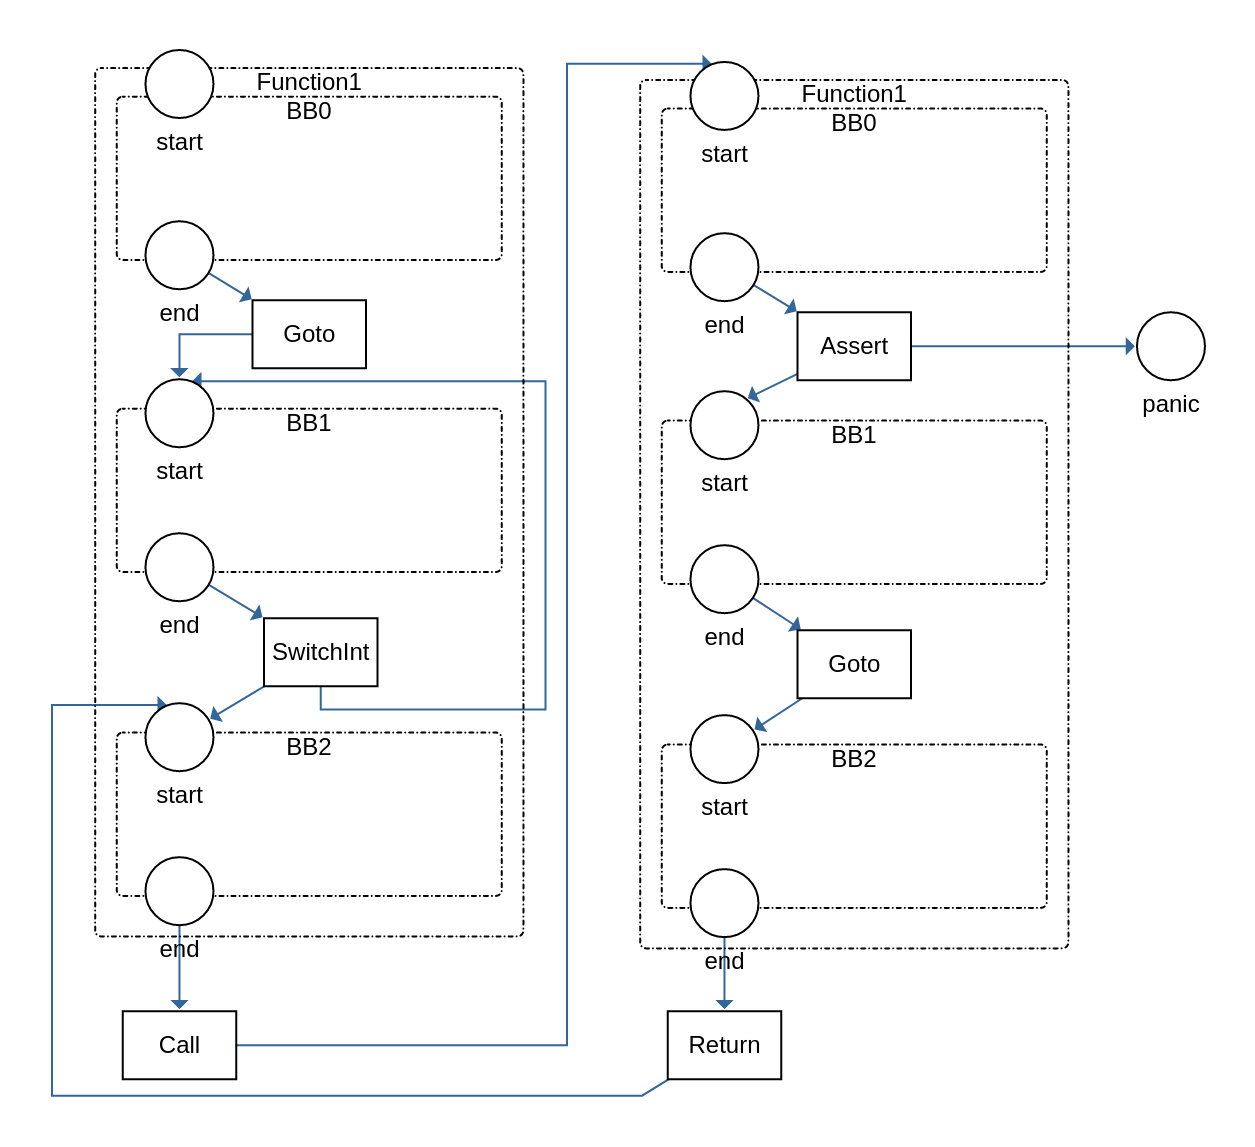
\includegraphics[width=.9\textwidth]{../diagrams/TerminatorsNet.png}
    \caption{Connection of terminator transitions}
    \label{terminators_net}
\end{figure}

We can see that terminators determine successful and unsuccessful execution causing panics which are a error handling mechanic of rust.
This is an important part of program execution and demands a little closer look.

\section{Panic Handling}
Error handling is a vital part in programming and typically is considered in program language design.
Many languages implement an exception semantic with try and catch blocks.
Exceptions can be thrown and if they are not catched the program terminates ungraceful.

Rust has a different approach: normally functions are expected to not fail.
Functions that can failed will return a \textit{Result} type that can be the result of the computation or an error with a description.
The type system enforces handling of both cases and the language gives some mechanisms to do so.
Of course the interesting part is the error case.
This one can be escalated to previous function calls until a consistent program state can be restored.

But it might not always be possible to recover from an error state.
In such a situation the program can be instructed to \textit{panic} and shutting down ungracefully like with an uncatched exception in other languages.
The programm execution is aborted, the stack will be unwinded and an error message with the details of the panic is generated (stating the error message and the location of the error).
Though, panics can be catched by a parent thread they typically lead to the termination of the current program.
This panic structure ensures that the compiler always knows when a panic can happen so it can generates appropriate code.

Code that we can identify and handle in the MIR representation.
We hinted this in the last chapter: some terminators can branch execution to a normal path or a panic path.
Branches to a panic path lead to basic blocks that are marked as cleanup and handle stack unwinding.
If execution enters a cleanup path, it cannot return to a normal path and will end up in an erroneous termination (unless catched by a parent thread).
We can model a separate termination place in our Petri-Net for this event.
This way we can check for this property later.
However, stack unwinding will execute generated code that is not a distinct part of the program semantic.
After all, what really matters is that an erroneous state was reached that we can't recover.
So we can reduce the size of our net by skipping the cleanup paths and directly put a mark on the panic place.

Of course the rust compiler cannot cast black magic to prevent the really bad errors like dereferencing pointers to unaccessible memory.
Such a miscalculation would lead directly to an os exception (or other undefined behavior) causing an error that cannot be catched by rust -- or worse -- a messed up state with no error at all!
And since rust cannot detect those errors, we cannot model them either.
We just have to assume that all compiled operations are valid in the execution context.

This kind of errors have to be avoided by the implementor.
But rust aids avoidance by marking such operations and functions as \textit{unsafe} to use.
Most of the time it is possible to avoid unsafe code using abstractions and safe operations.
Only a small code base needs to use unsafe code to create those safe abstractions and once the integrity there is kept, all depending higher level code benefits.

%TODO: überleitung

\section{Interface Emulation}
There are endless possibilities to implement an algorithm and not all of them depend on rust as description language.
Still, using established algorithms from other source languages is a desireable feature to have.
Unsurprisingly, rust implements some interfaces to access functionality that is not native to rust.
The two most important are compiler \textit{intrinsic functions} where the implementation is hidden by the compiler;
And the \textit{Foreign Function Interface} for interfacing C-Style exports.
Both of them call instructions that are not represented in the MIR graph.

These calls leave the realm of rust code where no guarantees can be made (which makes most of them unsafe).
But on lower level code we won't get around them.
For example rusts thread interface in linux systems is an abstraction of the `pthread' library which is written in C.
To translate such items we will have to emulate them somehow.
In case of compiler intrinsics this would be a finit amount of work but there is no upper bound for foreign functions that might be called.
So we have to implement at least a generic translation that works for all calls.
Additionally we can translate important functionality by hand.

A generic call can be thought of a combination of a statement and a terminator.
The locals for the arguments have to be accessed by a transition like we did for the statements.
Afterwards we branch depending on the return value, like we did in the terminators.
This behavior describes all basic data manipulation functionality.
But there are other functionalities that we need to address in a special way:
some foreign functionality can influence the execution flow.
For example mutexes and threads are significant for our purposes.

\subsection*{Mutexes}
Mutexes guard execution flow depending on a data variable.
If we just access the variable and continue like we do for statements, flow could always continue.
However, flow should only be allowed to continue if the mutex variable can be acquired (and block otherwise).
This can easily be modeled in Petri-Nets with a marked mutex place.
Then, on every try to acquire the mutex a transition has to consume the token from the mutex place.
The first try will do so without further problems but every following attempt will be blocked, since transitions can only fire when all pre-places are properly marked.
When leaving the critical section a transition needs to reproduce a mark on the mutex place again, so that blocked processes can continue with their computation.

%TODO: bild!
In rust Mutexes are part of the standard library.
Before data guarded by a mutex can be mutated it has to be unlocked.
If it is, the data cannot be accessed again until the lock is released.
This is done automatically when the variable of the accessed data goes out of scope.
listing \ref{rust-mutex} shows an example usage of a mutex.

\lstset{language=Rust,caption={Mutex in rust},label=rust-mutex, frame=none, stepnumber=5, backgroundcolor=\color{verylightgray}}
\begin{lstlisting}
use std::sync::{Arc, Mutex};

// Here we're using an Arc (reference counting smart pointer)
// to share memory among threads, and the data inside the Arc
// is protected with a mutex.
let data = Arc::new(Mutex::new(0));
{ // begin of a new scope
    // Mutex is acquired by the lock() method.
    // If the lock was previously acquired the call will block
    // until the lock is released
    let mut data: Arc<Mutex<i32>>= *data.lock().unwrap();
    // mutate data
    data += 1;
    // the lock is released here when `data` goes out of scope.
} // end of scope
\end{lstlisting}

Now, the call to mutex \textit{lock()} und the release of the the lock will trigger several other functions that handle a thread safe access and the blocking behavior.
For translation we can model the complete underlying behavior or abstract from it.
Both approaches are perfectly valid: the former would be closer to the actual execution behavior while the latter would be closer to the basic program semantics (that does not care about the mutex implementation).
But in favor of a small Petri-Net we stick to the abstract wa that ignores the implementation.
When a mutex is called we will stall normal execution and just insert our own abstraction at the place of the corresponding function calls.
But there is more we have to consider.

If we take a look on a pruned version of the MIR layer in listing \ref{rust-mutex-mir} we can identify a Problem.
Because mutexes are unlocked implicitly and often are wrapped in other types, we loose the information when a specific mutex is locked or unlocked.
The mutex that is created in \textit{bb0} is wrapped in a smart pointer in \textit{bb2} masking the original mutex.
In this simple program the smart pointer is unnecessary but usually mutexes guard critical sections to ensure thread safety.
However to reference the mutex safely in multiple threads the reference has to be thread safe, which is ensured by the wrapping \textit{Arc} smart pointer.
By the time we lock the mutex in \textit{bb4} we can not read directly from the local which mutex it belongs to (in case there are multiple mutexes in a program).
The same problem is inherited bey the mutex guard in local \textit{\_3}.

\lstset{language=Rust, caption={Pruned MIR for using a mutex},label=rust-mutex-mir, frame=none, stepnumber=5, backgroundcolor=\color{verylightgray}}
\begin{lstlisting}

fn  main() -> () {
    let mut _0: ();
    let _1: Arc<Mutex<i32>>;
    let mut _2: Mutex<i32>;
    let mut _4: &Mutex<i32>;
    let _5: &Mutex<i32>;
    let mut _6: &Arc<Mutex<i32>>;
    scope 1 {
        let _3: Result<MutexGuard<i32>, PoisonError<MutexGuard<i32>>>; 
    }
    // create the mutex first
    bb0: {
        _2 = const Mutex::<i32>::new(const 0i32) -> bb2; 
    }
    // move the mutex into the smart pointer
    bb2: {
        _1 = const Arc::<Mutex<i32>>::new(move _2) -> bb3; 
    }
    // dereference the smart pointer
    bb3: {
        _6 = &_1;                        
        _5 = const <Arc<Mutex<i32>> as deref(move _6) 
             -> [return: bb4, unwind: ...]; 
    }
    // lock the mutex
    bb4: {
        _4 = _5;                         
        _3 = const Mutex::<i32>::lock(move _4) 
             -> [return: ..., unwind: ...]; 
    }
    // mutex goes out of scope and destructor is called
    bb6: {
        drop(_3) -> [return: ..., unwind: ...];
    }
}
\end{lstlisting}

To connect our transitions to the correct mutex places we have to track or infer the corresponding mutexes when they are locked or unlocked.
In theory the strict borrowing and aliasing rules of rust should ensure that the correct mutex can always be inferred.
However, this is not trivial; So in the test implementation the local variables that are associated with a mutex (like the Arc in local \_1 and the MutexGuard in local \_3) are marked with the original mutex.
Locking and unlocking mutexes then just check the mark for the fitting mutex and connect its mutex places with the correct transitions.
This is a simple approach for a proof of concept, but it probably can be improved especially in storage consumption.

\section{Petri Net Representation}
\label{app_petri}
Implementing a basic graph structure to represent our Petri-Net is not very difficult.
But to be compatible with a Model checker we have to use some interface or a standard that
defines a commonly known structure.
Luckily there exists an xml-based standard for Petri-Nets called \textbf{Petri Net Markup Language}\cite{pnml}\cite{kindler2006petri} or \textbf{PNML}.
However, LoLa -- the model checker that we actually used -- defines it own representation.
And a third representation that comes in handy for visualizing and debugging is \textbf{DOT}\cite, a simple language for graph definitions.
All langauges are comparable in their core idea.
They all list nodes (places, transitions) and arcs of the graph. 
Additionally, the petri net representations encode information for token count and arc weight.
Since all the three representation serve their own perpose, they there all integrated as target representation in our work.
And with a finished translation we can finally feed a model checker with our Petri-Net.

\section{Model Checking}
\label{app_mc}
To test and inspect our results we have the choice between different tools.
%TODO: Tool liste
There are jada jada \cite .
For a proof of concept it is not very important which model checker is used, since we will verify small test programs;
Performance is not the biggest concern at this time.
This is why LoLa was chosen by personal preference for this work.

Having a model checker and a rust program that is translated to a Petri-Net, the last thing we need is a property to check for.
We want to search for deadlocks in the source program.
That means that the program execution is blocked unexpectedly and no operation can be executed.
This translates nicely a dead Petri-Net where no transition is active and the net reached a final state.
We have to be carful though: there are states where the Petri-Net is expectedly dead;
Program termination is by definition a state there execution stops.
This means that if we reach either the \textit{program end} or the \textit{panic} place, our net is expected to be dead.
To check for a unexpected deadlock we need to make sure that our termination places are not marked: $program\_end = 0\ \&\ panic = 0$.
Additionally the net has to be dead.
In LoLa this is expressed with the key word $DEADLOCK$.
So the state we want to discover would be $DEADLOCK\ \& (program\_end = 0\ \&\ panic = 0)$.
The final part we have to consider is the temporal aspect.
To specify that our state property holds eventually and to find an applicable path, we can use the $EF$ operator.
Its semantic is that the given property exists and will holds true at some point in the future.
So our final formula would look like this:
$$ EF(DEADLOCK\ \& (program\_end = 0\ \&\  panic = 0))$$
And having that, lets use it in a test program.

\section{Test Programs}
\label{app_test}
If we want to get some confidence in our translation we have to see if it behaves as expected.
Initially, the basic functionality should be testet against the most simple programs to fail early.
And what could be simpler than the empty program?
\lstset{language=Rust,caption={The empty program},label=empty-program, frame=none, stepnumber=5, backgroundcolor=\color{verylightgray}}
\begin{lstlisting}
pub fn main() {}
\end{lstlisting}
Beside giving a good starting point for a testable implementation, this program already revealed the edge case of empty functions.
These function are not necessarily optimized away on the MIR level but also have no basic blocks as expected for every other function;
A case that has to be considered.
Additionally, the fact that all terminating programs have a deadlock should also get obvious here at the latest!

Other programs that can strengthen the confidence in the translation process include some important language features, like an endless program (which actually is completely deadlock free):
\lstset{language=Rust,caption={An endless program},label=endless-program, frame=none, stepnumber=5, backgroundcolor=\color{verylightgray}}

\begin{lstlisting}
pub fn main() -> ! {
    loop {}
}
\end{lstlisting}
Or a program with a function call:

\lstset{language=Rust,caption={A simple function call},label=function_call_program, frame=none, stepnumber=5, backgroundcolor=\color{verylightgray}}
\begin{lstlisting}
pub fn main() {
    let mut x = 5;
    x = call(x);
}

fn call(i: usize) -> usize {
    i * 2
}
\end{lstlisting}

However, non of these programs are significant for what we really want to achieve: deadlock detection.
For this, we need a program that forces a repeating lock of a mutex.
This does not necessarily have to be in multiple threads
(which is fortunate since we did not cover actual parallelism with threads yet).
We simply have to lock the mutex twice in a row to create a deadlock.
And since the rust compiler does no own deadlock analisis this code compiles successfully:

\lstset{language=Rust,caption={A deadlock!},label=deadlock_program, frame=none, stepnumber=5, backgroundcolor=\color{verylightgray}}
\begin{lstlisting}
use std::sync::{Arc, Mutex};

pub fn main() {
    let data = Arc::new(Mutex::new(0));
    let data = Mutex::new(0);
    let _d1 = data.lock();
    let _d2 = data.lock(); // cannot lock, since d1 is still active
}// unreachable end of main
\end{lstlisting}
If our Petri-Net model is worth something it should detect a deadlock for this program and none if we remove the last line.

And with this we have all we need to evaluate our approch.

% \section{Debugging}
% \label{app_debug}
% \begin{verbatim}
% - dot file for small programms
% - finding unconnected nodes
%     - possible bug found
%     - marking live places as result
%     - uninitialized places still have to be marked
%       (or removed entirely)
% - witness path
%     - reducing the complicated net to witness path nodes 
%       and its neighbors
% \end{verbatim}